\begin{itemize}
    \item Nested query is when you use multiple select statements within select statements to get specific information.
    \item Find names of all employees who have sold over 30,000 to a single client:
        \begin{minted}[autogobble]{sql}
            SELECT employee.first_name, employee.last_name, employee.emp_id
            FROM employee 
            WHERE employee.emp_id IN(
                    SELECT works_with.emp_id 
                    FROM works_with 
                    WHERE works_with.total_sales > 30000
            );
        \end{minted}
        \begin{figure}[H]
            \centering
            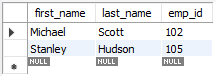
\includegraphics[width=0.4\textwidth]{./Figs/2020-12-24-21-51-11.png}
        % 	\caption{}
        \end{figure}
    
    \item Find all clients who are handled by the branch that Michael Scott manages, Assume you know Michael's ID.
        \begin{minted}[autogobble]{sql}
            SELECT client.client_name 
            FROM client 
            WHERE client.branch_id = (
                SELECT branch.branch_id 
                FROM branch 
                WHERE branch.mgr_id = 102
                LIMIT 1
            );
        \end{minted}
        \begin{figure}[H]
            \centering
            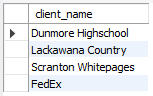
\includegraphics[width=0.4\textwidth]{./Figs/2020-12-24-21-51-49.png}
        % 	\caption{}
        \end{figure}
\end{itemize}
